\chapter{System Architecture}

\begin{figure}[h]
	\centering
	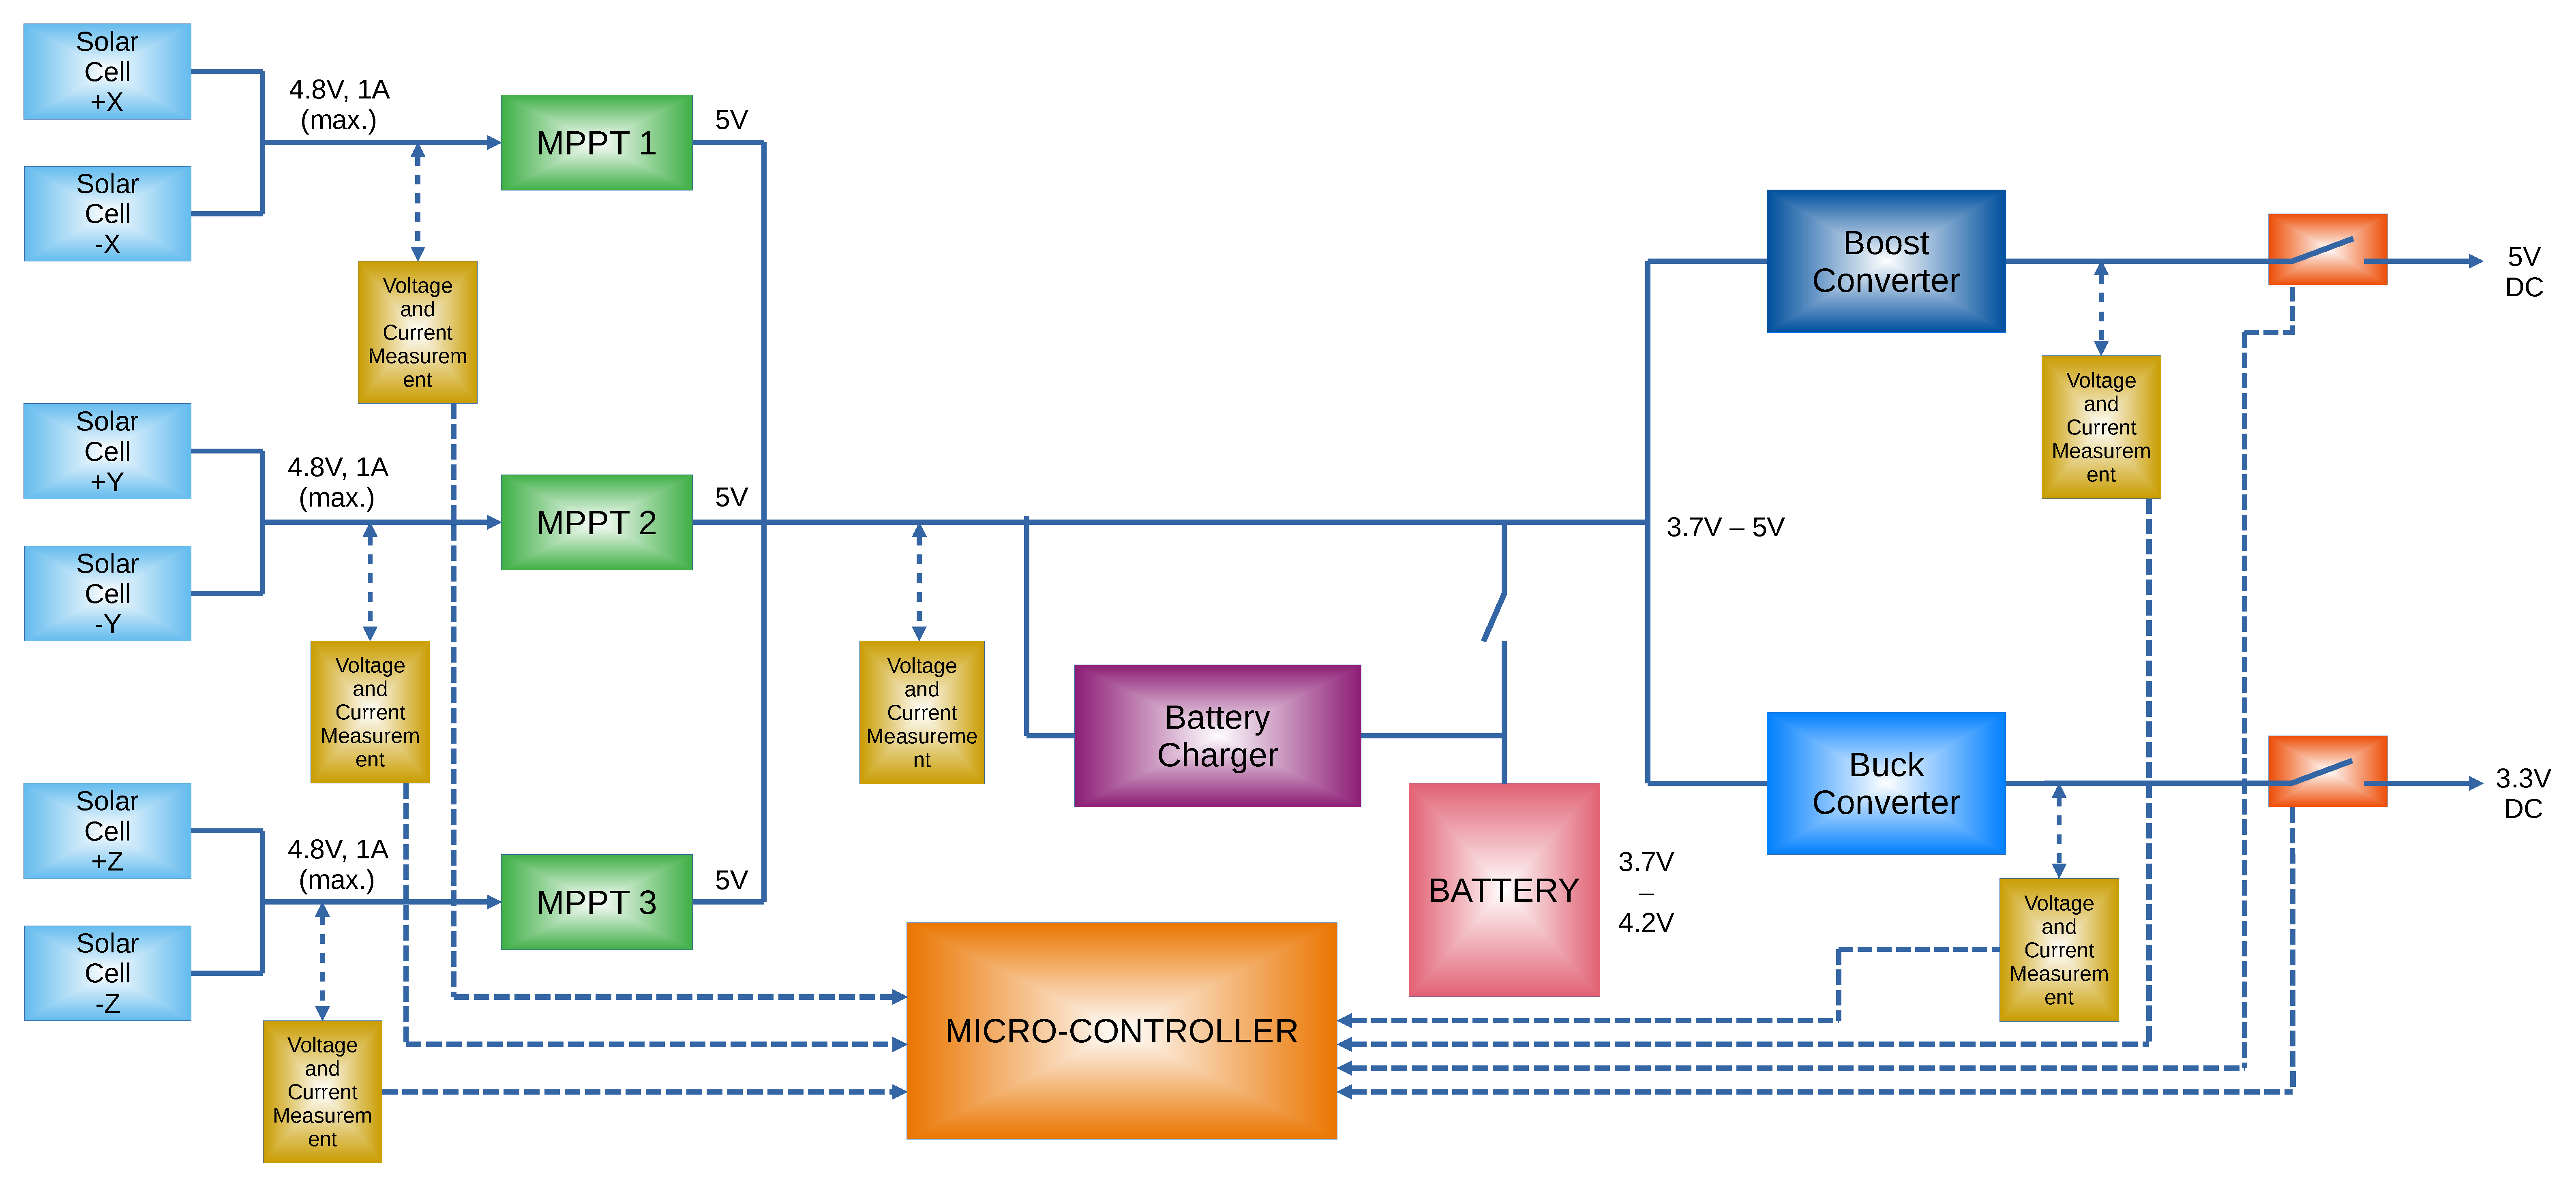
\includegraphics[width=\columnwidth]{diag1.pdf}
	\caption{System Architecture of the CubeSat EPS}
	\label{fig:arch}
\end{figure} 

The CubeSat is equipped with six solar panels on each side. To ensure that the solar panels operate at their most efficient points, the solar panels are connected to MPPT ICs such that the solar panels on the opposite sides are connected to single MPPT IC. Since only one of the opposite sides of the cube is irradiated at any time, the MPPT of two solar panels can be achieved using a single IC. This arrangement reduces the number of MPPT ICs required by the system. The MPPT runs a constant voltage algorithm and delivers 5V at the bus. 
\\

When the CubeSat is capable of generating enough power through the solar panels, the components are directly powered by the panels through the bus. At the same time, a battery charging IC uses some of the energy to recharge the Li-ion cell. The battery charger takes the 5V from the bus and converts it to the voltage and current optimal for battery charging depending on the state of charge, temperature of the cell etc.During eclipse the battery power the energy from the panels is absent and the battery powers the CubeSat components. The voltage of the battery varies from 3.7V to 4.2V.
\\

The buck and boost converters provide power to the 3.3V and 5V rails respectively. Their input voltage varies from 3.6V to 5V to account for direct power from the panels when sunlight is available and for battery power during eclipse.
\\

To ensure proper functioning and to identify any faults in the system, there are various voltage and current measurement units placed at various points in the circuit. They measure the current and voltage at each point and the data is fed to a micro-controller, which is programmed to open the switches at the rails in case of any faults.